Blake2~\cite{blake2} is a cryptographic hash and \gls{mac}. It is faster than
\emph{MD5}, \emph{SHA-1}, \emph{SHA-2} and \emph{SHA-3}, but is at least as
secure as the latest standard \emph{SHA-3}.
It comes in two flavors:
\begin{itemize}
	\item \emph{Blake2B} is optimized for $64$-bit platforms and produces
		digests of any size between $1$ and $64$ bytes
	\item \emph{Blake2S} is optimized for $8$- to $32$-bit platforms and
		produces digests of any size between $1$ and $32$ bytes.
\end{itemize}

A hardware implementation was created by Benedikt Tutzer and Dinka Milovancev as
part of the \emph{Digital Integrated Circuits} Laboratory at TU
Wien~\cite{blake2hardware}.
Even though we are working on a $32$-bit platform, we chose to implement
Blake2B, since at hardware level we can chose what bit-width to use.

The core is added to the system design as described in
\Cref{ssec:zynqhardwaredesign} and given the address $0x7E410000$. A size of
$64K$ is sufficient.
\gls{xps} generates the needed files in
\emph{<repo>hardware\_design/pcores/blake2b\_v1\_00\_a}.
The files from~\cite{blake2hardware} are then added to the vhdl-source directory
of the core,\\
\emph{<repo>/hardware\_design/pcores/blake2b\_v1\_00\_a/hdl/vhdl}.
\gls{xps} needs to be made aware of the additional files, otherwise they will be
left out of the synthesis flow.
To include them, the \gls{pao} file of the core, found in
\emph{<repo>/hardware\_design/pcores/blake2b\_v1\_00\_a/data/blake2b_v2_1_0.pao},
needs to be adapted accordingly:

\begin{lstlisting}[
	language=Bash,
	caption={\gls{pao} file of the blake2b core},
	label={lst:mpdblake},
	basicstyle=\small,
	float=h,
	floatplacement=h
	]
lib proc_common_v3_00_a  all 
lib axi_lite_ipif_v1_01_a  all 
lib blake2b_v1_00_a blake2 vhdl
lib blake2b_v1_00_a blake2b_wrapper vhdl
lib blake2b_v1_00_a user_logic vhdl
lib blake2b_v1_00_a blake2b vhdl
\end{lstlisting}

The entity from~\cite{blake2hardware} needs to be wrapped in the user\_logic.vhd
file.
It was configured to have $4$ software accessible registers, each $32$-bit wide:

\begin{tabular}{ll}
	Address & Name \\
	base     & task\_reg\\
	base + 4 & message\_reg\\
	base + 8 & status\_reg\\
	base + 16 & hash\_reg\\
\end{tabular}

With interface generated by the Xilinx tools, the core is only able to react to
register reads or -writes from the software.
It cannot send interrupt to the software.
To add this functionality, an additional port, of type \emph{std\_logic} is
added added and routed through the wrapper in \emph{blake2b.vhd} so that it is
visible as an output port of the peripheral.
It is called \emph{Interrupt}.
To have it act as an interrupt signal, it has to be declared as such in the
cores \gls{mpd} file,
\emph{<repo>/hardware_design/pcores/blake2b_v1_00_a/data/blake2b\_v2\_1\_0.mpd}.
This is done with the following lines:

\begin{lstlisting}[
	language=Bash,
	caption={Configure output port as interrupt},
	label={lst:interruptmpd},
	basicstyle=\small,
	float=h,
	floatplacement=h
	]
PARAMETER C_INTERRUPT_PRESENT = 1, DT = INTEGER, RANGE = (0,1)
PORT Interrupt = "", DIR = O, SIGIS = INTERRUPT, SENSITIVITY = EDGE_RISING, INTERRUPT_PRIORITY = MEDIUM, ISVALID = (C_INTERRUPT_PRESENT == 1)
\end{lstlisting}

The port then shows up as an interrupt port.
To connect it to the \gls{gic}, one must select the Zynq tab and click on the
\emph{IRQ} table as seen in \Cref{fig:gic}.

\begin{figure}[h]
\centering
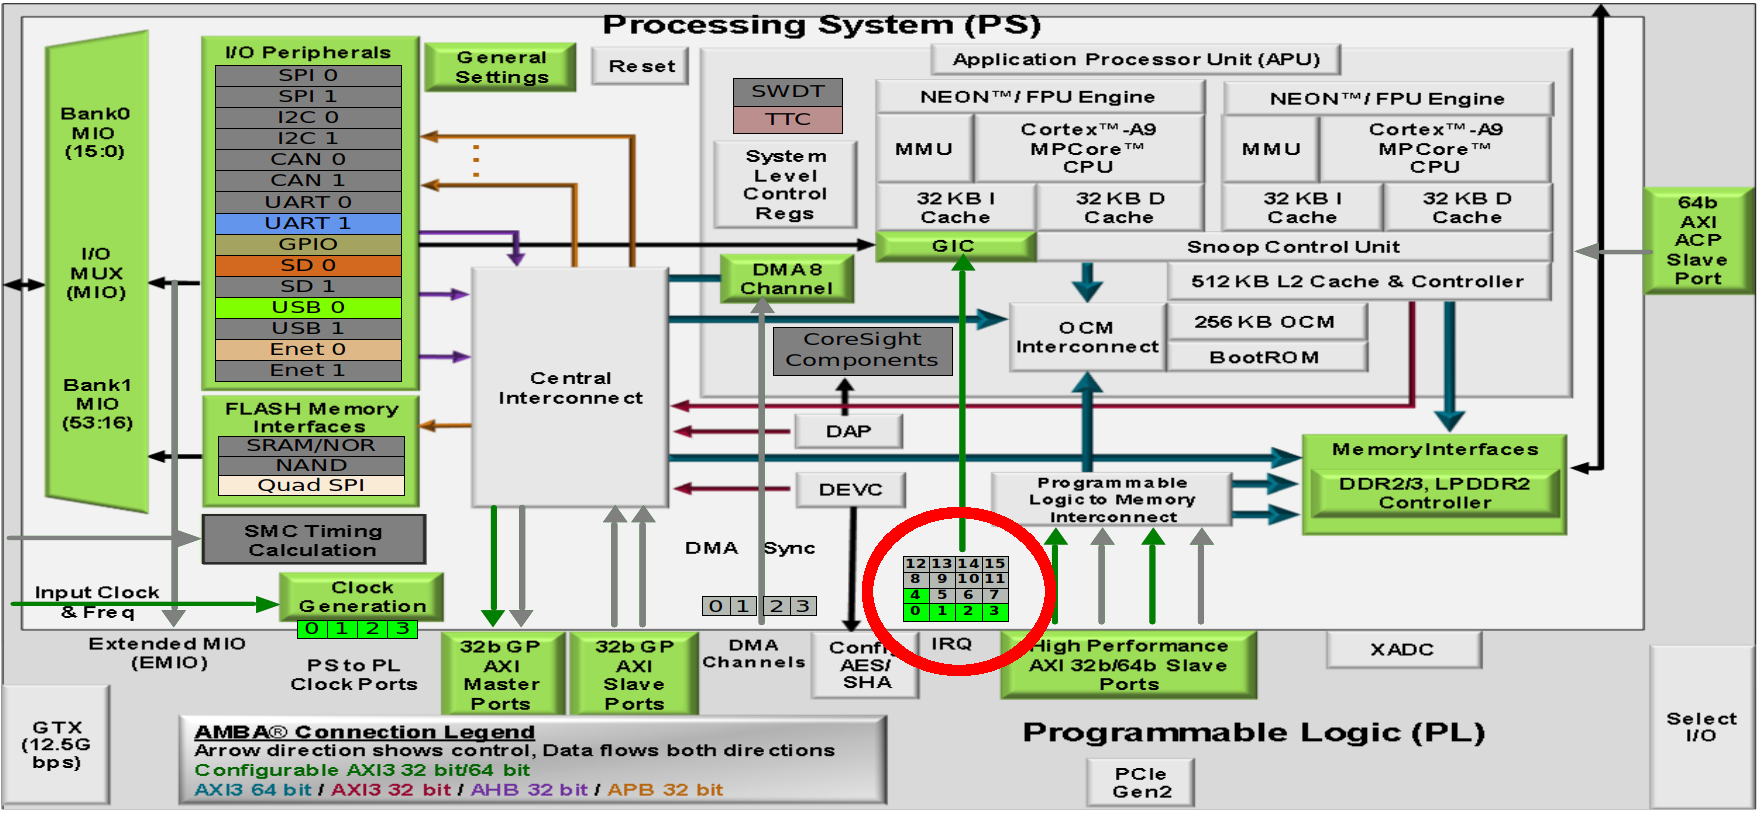
\includegraphics[width=1\textwidth]{sections/methodology/gic}
\caption{\label{fig:gic} IRQ table in the Zynq tab}
\end{figure}

On the upcoming dialog, the interrupt signal is shown as unconnected interrupt
in the left column.
By selecting it and clicking the arrow that points to the right it can be moved
to the right and is then connected, as seen in \Cref{fig:gicconnect}.

\begin{figure}[h]
\centering
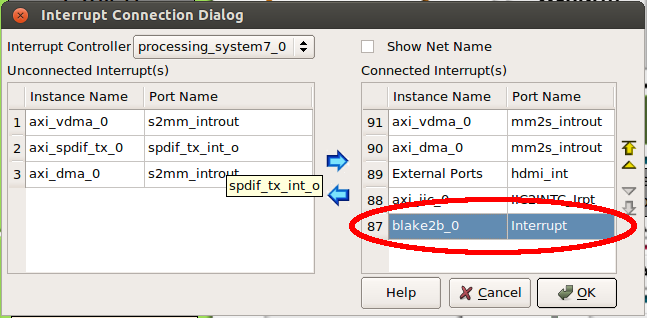
\includegraphics[width=1\textwidth]{sections/methodology/gicconnect}
\caption{\label{fig:gicconnect} Interrupt Connection Dialog}
\end{figure}

The number shown on the left side of the right column, $87$ in this example, is
the interrupt number that the device driver will have to connect to.
This can be seen in \Cref{sssec:linuxkernelmodules}.

The protocol how this device communicates with the device driver is simple.
To hash data, it has to be split into chunks of $32$-bits as the registers are
only $32$ bits wide.
The following steps need to be followed to hash data:
\begin{enumerate}
	\item Driver writes number of bytes to be hashed to the task register
	\item If all the data was sent, go to \Cref{item:end}\label{item:check}
	\item Device raises interrupt to signal that more data is needed
	\item Driver catches interrupt and writes a chunk of data to the message
		register
	\item Go to \Cref{item:check}
	\item Device raises interrupt to signal that hashing is done\label{item:end}
\end{enumerate}
The hash is always $64$-bytes long, so to read it back to the driver it has to
be split into $16$ individual $32$-bit chunks.
To read the hash from the device, the following steps are done:
\begin{enumerate}
	\item Driver iterates over $16$ hash chunks
		\begin{enumerate}
			\item Driver writes index of hash-chunk to status register
			\item Devices places the according chunk onto the hash register
			\item Driver reads hash register
		\end{enumerate}
	\item Driver concatenates hash chunks
\end{enumerate}
